\documentclass[crop,tikz]{standalone} 
\usepackage{tikz, amsmath, amssymb, graphicx} 

\DeclareMathAlphabet\mathbfcal{OMS}{cmsy}{b}{n}

\newcommand{\Mt}{\mathbfcal{M}}
\newcommand{\Yt}{\mathbfcal{Y}}
\newcommand{\Ft}{\mathbfcal{F}}

\usetikzlibrary{positioning, shapes.geometric} 

\begin{document} 

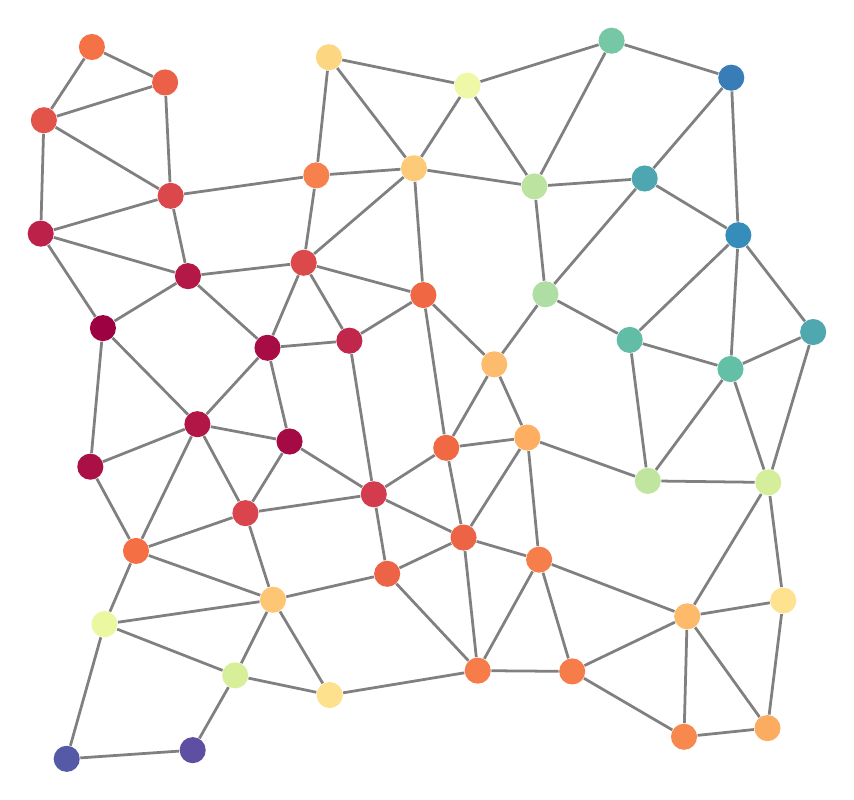
\begin{tikzpicture} 


\tikzstyle{node_style} = [circle,draw=blue!40!,fill=blue!20!, line width=1]
\tikzstyle{edge_style} = [draw=gray, line width=1]


\node[circle, fill={rgb,255:red,246; green,126; blue,75}] (v0) at (6.37, 2.70) {};
\node[circle, fill={rgb,255:red,192; green,229; blue,159}] (v1) at (7.75, 3.70) {};
\node[circle, fill={rgb,255:red,246; green,124; blue,74}] (v2) at (5.59, 1.29) {};
\node[circle, fill={rgb,255:red,237; green,99; blue,69}] (v3) at (4.44, 2.52) {};
\node[circle, fill={rgb,255:red,253; green,174; blue,97}] (v4) at (6.22, 4.25) {};
\node[circle, fill={rgb,255:red,241; green,105; blue,67}] (v5) at (5.19, 4.12) {};
\node[circle, fill={rgb,255:red,246; green,124; blue,74}] (v6) at (6.79, 1.28) {};
\node[circle, fill={rgb,255:red,253; green,186; blue,107}] (v7) at (8.25, 1.98) {};
\node[circle, fill={rgb,255:red,247; green,137; blue,79}] (v8) at (8.21, 0.45) {};
\node[circle, fill={rgb,255:red,213; green,238; blue,155}] (v9) at (9.28, 3.68) {};
\node[circle, fill={rgb,255:red,99; green,191; blue,165}] (v10) at (8.80, 5.12) {};
\node[circle, fill={rgb,255:red,97; green,189; blue,166}] (v11) at (7.52, 5.49) {};
\node[circle, fill={rgb,255:red,254; green,226; blue,143}] (v12) at (9.47, 2.18) {};
\node[circle, fill={rgb,255:red,240; green,103; blue,68}] (v13) at (4.90, 6.06) {};
\node[circle, fill={rgb,255:red,211; green,60; blue,78}] (v14) at (4.27, 3.53) {};
\node[circle, fill={rgb,255:red,192; green,39; blue,74}] (v15) at (3.96, 5.48) {};
\node[circle, fill={rgb,255:red,166; green,10; blue,68}] (v16) at (3.20, 4.20) {};
\node[circle, fill={rgb,255:red,252; green,172; blue,96}] (v17) at (9.27, 0.56) {};
\node[circle, fill={rgb,255:red,79; green,168; blue,175}] (v18) at (9.85, 5.59) {};
\node[circle, fill={rgb,255:red,55; green,141; blue,186}] (v19) at (8.90, 6.82) {};
\node[circle, fill={rgb,255:red,174; green,222; blue,163}] (v20) at (6.45, 6.07) {};
\node[circle, fill={rgb,255:red,220; green,73; blue,75}] (v21) at (3.38, 6.47) {};
\node[circle, fill={rgb,255:red,253; green,188; blue,109}] (v22) at (5.80, 5.18) {};
\node[circle, fill={rgb,255:red,188; green,228; blue,160}] (v23) at (6.31, 7.44) {};
\node[circle, fill={rgb,255:red,253; green,202; blue,120}] (v24) at (4.78, 7.67) {};
\node[circle, fill={rgb,255:red,246; green,129; blue,76}] (v25) at (3.54, 7.58) {};
\node[circle, fill={rgb,255:red,219; green,72; blue,76}] (v26) at (1.69, 7.32) {};
\node[circle, fill={rgb,255:red,168; green,12; blue,68}] (v27) at (2.92, 5.39) {};
\node[circle, fill={rgb,255:red,179; green,24; blue,71}] (v28) at (1.91, 6.30) {};
\node[circle, fill={rgb,255:red,77; green,166; blue,176}] (v29) at (7.71, 7.54) {};
\node[circle, fill={rgb,255:red,253; green,214; blue,130}] (v30) at (3.70, 9.08) {};
\node[circle, fill={rgb,255:red,239; green,248; blue,167}] (v31) at (5.46, 8.72) {};
\node[circle, fill={rgb,255:red,253; green,198; blue,117}] (v32) at (2.99, 2.19) {};
\node[circle, fill={rgb,255:red,254; green,225; blue,141}] (v33) at (3.71, 0.98) {};
\node[circle, fill={rgb,255:red,237; green,99; blue,69}] (v34) at (5.41, 2.98) {};
\node[circle, fill={rgb,255:red,217; green,68; blue,77}] (v35) at (2.64, 3.29) {};
\node[circle, fill={rgb,255:red,235; green,96; blue,70}] (v36) at (1.62, 8.76) {};
\node[circle, fill={rgb,255:red,188; green,34; blue,73}] (v37) at (0.04, 6.84) {};
\node[circle, fill={rgb,255:red,158; green,1; blue,66}] (v38) at (0.83, 5.64) {};
\node[circle, fill={rgb,255:red,226; green,83; blue,73}] (v39) at (0.08, 8.28) {};
\node[circle, fill={rgb,255:red,177; green,22; blue,70}] (v40) at (2.03, 4.42) {};
\node[circle, fill={rgb,255:red,94; green,79; blue,162}] (v41) at (1.97, 0.28) {};
\node[circle, fill={rgb,255:red,216; green,239; blue,154}] (v42) at (2.51, 1.23) {};
\node[circle, fill={rgb,255:red,170; green,15; blue,69}] (v43) at (0.67, 3.88) {};
\node[circle, fill={rgb,255:red,244; green,114; blue,69}] (v44) at (0.69, 9.21) {};
\node[circle, fill={rgb,255:red,235; green,247; blue,161}] (v45) at (0.85, 1.88) {};
\node[circle, fill={rgb,255:red,85; green,90; blue,167}] (v46) at (0.37, 0.17) {};
\node[circle, fill={rgb,255:red,244; green,111; blue,68}] (v47) at (1.25, 2.81) {};
\node[circle, fill={rgb,255:red,57; green,125; blue,184}] (v48) at (8.81, 8.82) {};
\node[circle, fill={rgb,255:red,118; green,200; blue,164}] (v49) at (7.29, 9.29) {};

\draw[edge_style] (v2) edge (v0);
\draw[edge_style] (v3) edge (v2);
\draw[edge_style] (v4) edge (v0);
\draw[edge_style] (v4) edge (v1);
\draw[edge_style] (v5) edge (v4);
\draw[edge_style] (v6) edge (v0);
\draw[edge_style] (v6) edge (v2);
\draw[edge_style] (v7) edge (v0);
\draw[edge_style] (v7) edge (v6);
\draw[edge_style] (v8) edge (v6);
\draw[edge_style] (v8) edge (v7);
\draw[edge_style] (v9) edge (v1);
\draw[edge_style] (v9) edge (v7);
\draw[edge_style] (v10) edge (v1);
\draw[edge_style] (v10) edge (v9);
\draw[edge_style] (v11) edge (v1);
\draw[edge_style] (v11) edge (v10);
\draw[edge_style] (v12) edge (v7);
\draw[edge_style] (v12) edge (v9);
\draw[edge_style] (v13) edge (v5);
\draw[edge_style] (v14) edge (v3);
\draw[edge_style] (v14) edge (v5);
\draw[edge_style] (v15) edge (v13);
\draw[edge_style] (v15) edge (v14);
\draw[edge_style] (v16) edge (v14);
\draw[edge_style] (v17) edge (v7);
\draw[edge_style] (v17) edge (v8);
\draw[edge_style] (v17) edge (v12);
\draw[edge_style] (v18) edge (v9);
\draw[edge_style] (v18) edge (v10);
\draw[edge_style] (v19) edge (v10);
\draw[edge_style] (v19) edge (v11);
\draw[edge_style] (v19) edge (v18);
\draw[edge_style] (v20) edge (v11);
\draw[edge_style] (v21) edge (v13);
\draw[edge_style] (v21) edge (v15);
\draw[edge_style] (v22) edge (v4);
\draw[edge_style] (v22) edge (v5);
\draw[edge_style] (v22) edge (v13);
\draw[edge_style] (v22) edge (v20);
\draw[edge_style] (v23) edge (v20);
\draw[edge_style] (v24) edge (v13);
\draw[edge_style] (v24) edge (v21);
\draw[edge_style] (v24) edge (v23);
\draw[edge_style] (v25) edge (v21);
\draw[edge_style] (v25) edge (v24);
\draw[edge_style] (v26) edge (v25);
\draw[edge_style] (v27) edge (v15);
\draw[edge_style] (v27) edge (v16);
\draw[edge_style] (v27) edge (v21);
\draw[edge_style] (v28) edge (v21);
\draw[edge_style] (v28) edge (v26);
\draw[edge_style] (v28) edge (v27);
\draw[edge_style] (v29) edge (v19);
\draw[edge_style] (v29) edge (v20);
\draw[edge_style] (v29) edge (v23);
\draw[edge_style] (v30) edge (v24);
\draw[edge_style] (v30) edge (v25);
\draw[edge_style] (v31) edge (v23);
\draw[edge_style] (v31) edge (v24);
\draw[edge_style] (v31) edge (v30);
\draw[edge_style] (v32) edge (v3);
\draw[edge_style] (v33) edge (v2);
\draw[edge_style] (v33) edge (v32);
\draw[edge_style] (v34) edge (v0);
\draw[edge_style] (v34) edge (v2);
\draw[edge_style] (v34) edge (v3);
\draw[edge_style] (v34) edge (v4);
\draw[edge_style] (v34) edge (v5);
\draw[edge_style] (v34) edge (v14);
\draw[edge_style] (v35) edge (v14);
\draw[edge_style] (v35) edge (v16);
\draw[edge_style] (v35) edge (v32);
\draw[edge_style] (v36) edge (v26);
\draw[edge_style] (v37) edge (v26);
\draw[edge_style] (v37) edge (v28);
\draw[edge_style] (v38) edge (v28);
\draw[edge_style] (v38) edge (v37);
\draw[edge_style] (v39) edge (v26);
\draw[edge_style] (v39) edge (v36);
\draw[edge_style] (v39) edge (v37);
\draw[edge_style] (v40) edge (v16);
\draw[edge_style] (v40) edge (v27);
\draw[edge_style] (v40) edge (v35);
\draw[edge_style] (v40) edge (v38);
\draw[edge_style] (v42) edge (v32);
\draw[edge_style] (v42) edge (v33);
\draw[edge_style] (v42) edge (v41);
\draw[edge_style] (v43) edge (v38);
\draw[edge_style] (v43) edge (v40);
\draw[edge_style] (v44) edge (v36);
\draw[edge_style] (v44) edge (v39);
\draw[edge_style] (v45) edge (v32);
\draw[edge_style] (v45) edge (v42);
\draw[edge_style] (v46) edge (v41);
\draw[edge_style] (v46) edge (v45);
\draw[edge_style] (v47) edge (v32);
\draw[edge_style] (v47) edge (v35);
\draw[edge_style] (v47) edge (v40);
\draw[edge_style] (v47) edge (v43);
\draw[edge_style] (v47) edge (v45);
\draw[edge_style] (v48) edge (v19);
\draw[edge_style] (v48) edge (v29);
\draw[edge_style] (v49) edge (v23);
\draw[edge_style] (v49) edge (v31);
\draw[edge_style] (v49) edge (v48);


 
% \draw [green, dashed] (1, -2.7) rectangle (2.05, 0.3);

% \node [below, opacity=0, text opacity=1] at (2.45, -1) {$\otimes$};

% \draw [blue, dashed] (2.9, -2.7) rectangle (6.5, 0.3);
% \node[inner sep=0pt] (subjects) at (6.2, -0.2) {};

% \node [below, opacity=0, text opacity=1] at (6.9, -1) {$\otimes$};

% \draw [orange, dashed] (7.4, -2.7) rectangle (10.5, 0.3);
% \node[inner sep=0pt] (stimuli) at (10.3, -0.2) {\includegraphics[width=.22\textwidth]{fMRI_Stimuli_Diagram.pdf}};




\end{tikzpicture}
\end{document} 
